\setcounter{chapter}{3}
\chapter{Theories}

In this chapter,
we look at first-order theories:
sets of sentences in a formal, first-order language that are
assumed to describe a particular domain of objects.
Such a theory could describe the behaviour of physical systems
or moral norms,
but we'll focus on mathematical theories
-- specifically, arithmetic and set theory.

\section{Arithmetic}\label{sec:arithmetic}

For most of history,
people did maths in an informal manner,
relying on a loose collection of techniques for solving specific types of problems.
When giving proofs,
assumptions that seemed obviously true
-- for example, that $0 \ne 1$ --
were simply taken for granted.

In the 19th and early 20th century,
mathematics was put on a more rigorous footing.
Cauchy, Weierstrass, Dedekind, and others gave
precise definitions of mathematical concepts such as limits and continuity,
and formalized the exact assumptions that
were needed to derive well-known results.
% It now became possible to show
% that the techniques mathematicians had been using were indeed valid.

At the same time,
more powerful mathematical theories were developed,
such as the set theory of Cantor
(formalized by Zermelo, Fraenkel, and others),
or the type theory of Russell and Whitehead.
All known branches of maths,
it seemed,
could be unified in such a theory,
allowing for new results to be derived
from the emerging connections between previously separate domains.
Theorems from topology could be used to prove results in algebra.

Formally,
a \emph{theory} is a set of sentences that is closed under entailment,
so that it contains everything that is entailed by it.
In this chapter,
we'll be concerned with theories in a formal, first-order language.
We often write $\vdash_{T} A$ or $T \vdash A$  (rather than $A \in T$)
to say that a sentence $A$ is a member of the theory $T$.

This fits our earlier use of the turnstile:
If $A$ is in $T$,
then $T \vdash A$ (by Mon and Id);
conversely,
if $T \vdash A$,
then by the completeness of first-order logic,
$T \entails A$,
and then $A$ is in $T$ because $T$ is closed under entailment.
We could write $T \entails A$ instead of $T \vdash A$.
Conceptually, however,
theories belong to the ``syntax'' or ``proof theory'' side of logic.
A theory is simply a set of sentences.
This set is usually specified by laying down some non-logical axioms.
The theory then contains all and only the sentences
that can be derived from these axioms.
We say that a theory $T$ is \emph{axiomatized} by a set of sentences $\Gamma$
if it contains exactly the sentences that are derivable from $\Gamma$.

% [I could now introduce a simple theory, e.g. linear orders.]

\begin{exercise}
  Let $\L$ be some first-order language (with identity).
  Let $T_1$ be the theory axiomatized by the set of all $\L$-sentences,
  $T_2$ the theory axiomatized by the empty set of sentences,
  and $T_3$ the theory axiomatized by $\{ \forall x \, x\ne x \}$.
  Which of $T_1$, $T_2$, and $T_3$ are the same?
\end{exercise}


Let's take a closer look at formal theories of arithmetic.
Arithmetic is the study of the natural numbers 0, 1, 2, 3, etc.
We know a lot about the natural numbers.
We know, for example,
that $1+2=3$,
that there are infinitely many primes,
or that the factorial function $x!$ grows faster than any polynomial $x^n$.
% There are also things we don't know.
% We don't know if
% every even number greater than 2 is the sum of two primes
% (Goldbach's conjecture).
The aim of an axiomatized formal theory of arithmetic
is to capture all such truths,
showing exactly which assumptions (or axioms) are needed to derive which results.

An important part of the axiomatic project is to reduce the number of primitive concepts.
In section~\ref{sec:unintended},
I already mentioned that
we don't need separate individual constants for each number:
we can instead use a single constant `0' for the number 0
and a function symbol `$s$' for the successor function;
the number 1 is then denoted by `$s(0)$',
the number 2 by `$s(s(0))$', and so on.
This is useful because it means that
we don't need special axioms for each number:
having defined 1, 2, and 3 as $s(0)$, $s(s(0))$, and $s(s(s(0)))$,
respectively,
we may hope to derive that $1 + 2 = 3$
from general assumptions about zero and the successor function.
If `1', `2', and `3' were primitive symbols,
it is hard to see how `$1 + 2 = 3$' could be derived
from more basic principles.

In section~\ref{sec:unintended},
I suggested that a first-order theory of arithmetic
might use primitive symbols for 0,
the successor function,
addition,
multiplication,
and the less-than relation.
In fact,
the less-than relation can be defined in terms of the other concepts
and logical expressions,
since the following holds for all natural numbers $x$ and $y$:
\[
  x < y \text{ iff } \exists z (x + s(z) = y ).
\]
We can therefore treat `$t_1 < t_2$',
for any terms $t_1$ and $t_2$,
as a metalinguistic abbreviation of
`$\exists x ( t_1 + s(x) = t_2 )$'.
(The variable $x$ must not occurring in $t_1$ or $t_2$.)
%
% \begin{axioms}
%   & $t_{1} < t_{2}$ abbreviates $\exists x ( t_{1} + s(x) = t_{2} )$.
% \end{axioms}
%

Less obviously, we can define the concept of a prime number.
Remember that a number is prime if
it is greater than 1 and divisible only by 1 and itself.
A number $x$ is divisible by a number $y$
if there is a number $z$ such that $z \times y = x$.
Thus we can express `$t$ is prime' as:
\[
  s(0) < t \land \forall y(\exists z(z \times y = t) \to (y = s(0) \lor y = t)).
\]

\begin{exercise}
  Define the concepts of (a) an even number and (b) a square number.
\end{exercise}

% \begin{exercise}
%   Show that < is irreflexive and transitive.
% \end{exercise}

Other concepts are harder to define.
It is not obvious how one could
define exponentiation $x^y$ or the factorial $x!$ in terms of 0, $s$, $+$, and $\times$.
We'll see in chapter~\ref{ch:representability} how it can be done.
Indeed,
we'll see that
all computable functions and relations on the natural numbers
can be defined in terms of our four primitives.
That is,
whenever there is an algorithm for computing a function,
or for determining whether a relation holds between some numbers,
then the function or relation can be defined in terms of 0, $s$, $+$, and $\times$.

\begin{exercise}
  Can you find another primitive that we could use instead of `$s$'?
  (That is, can you find a primitive symbol $\varphi$ so that
  $s(t)$ can be defined from 0, $\varphi$, $+$, and $\times$?)
\end{exercise}

Let's turn to the second part of the axiomatic project.
Having reduced the set of primitive concepts,
we need to lay down axioms
that describe how the remaining concepts behave.
The aim is to reduce all truths about the natural numbers
to a small number of basic principles.

The first axioms we'll consider are just about 0 and $s$.
Later,
we'll add axioms for $+$ and $\times$.
What do we know about 0 and $s$?
We know, for example,
that every number has a successor.
But we don't need to postulate this as an axiom:
all function symbols in first-order logic denote total functions.
What isn't guaranteed is that
`$s$' denotes an injective function:
we need to postulate that
no two numbers have the same successor.

\begin{axioms}
  Q1 & $\forall x\forall y\, (s(x)\!=\!s(y) \,\to\, x\!=\!y)$ \\
\end{axioms}

We also know that 0 is not the successor of any number:

\begin{axioms}
  Q2 & $\forall x \, 0\! \not= \!s(x)$
\end{axioms}

These two axioms are already quite powerful.
Let's think about what a model of them must look like.
There must be at least one object,
denoted by 0.
There must also be an object $s(0)$.
Can this be the same as 0?
No:
otherwise 0 would be the successor of itself,
which contradicts Q2.
So $s(0)$ is another object.
What about $s(s(0))$?
This can't be 0, by Q2.
And so it can't be $s(0)$ either, by Q1:
if $s(s(0)) = s(0)$,
then $s(0)$ and $0$ would have the same successor.
So $s(s(0))$ is a third object.
By iterating this reasoning,
we can see that any model of Q1 and Q2 must have
a chain of infinitely many objects
\[
  0, s(0), s(s(0)), s(s(s(0))), \ldots,
\]
connected by the successor function.

\begin{exercise}\label{ex:q1q2}
  Can you find a model in which Q1 and Q2 are true,
  but $\forall x (s(x) \ne x)$ is false?
\end{exercise}

Exercise~\ref{ex:q1q2} shows that
Q1 and Q2 don't suffice to capture all truths about 0 and $s$.
The problem is that
the two axioms don't rule out the existence of other objects,
outside the chain $0, s(0), s(s(0)), \ldots$.
On these other objects,
the successor relation must still be injective,
but it can go in a loop,
or it can form a second infinite chain
$a, s(a), s(s(a)), \ldots$.
The following axiom to rule out such chains,
by stipulating that there is no object other than 0 that is not a successor.

\begin{axioms}
  Q3 & $\forall x \,(x\!\not= 0 \,\to\, \exists y\, x\!=\!s(y))$
\end{axioms}

This doesn't help with the looping case,
however.
Intuitively,
we'd like to have a postulate saying that
every number can eventually be reached from 0 by repeated application of $s$.
But there's no way to express this in first-order logic
(as we proved in section~\ref{sec:unintended}).
Still,
we can get close
by adding the following axiom schema,
called the \emph{induction schema}:

\begin{axioms}
  Ind & $(A(0) \land \forall x\; (A(x) \rightarrow A(s(x))) \to \forall x\; A(x))$
\end{axioms}

Here, $A(x)$ is any formula with one free variable.
Think of every such formula as expressing a property.
Ind then says that
if some (expressible) property holds of 0,
and if it is inherited from any number to its successor,
then it holds of all numbers.
The schema is obviously related to the method of inductive proof,
where we show that
all numbers have a property
by showing that 0 has it and that it is inherited from any number to its successor.

Ind rules out the looping case.
Consider the simplest version,
where there's an object $a$ outside the chain $0, s(0), s(s(0)), \ldots$
that is its own successor.
In this model,
$\forall x (s(x) \ne x)$ is false.
But $\forall x (s(x) \ne x)$ follows from Q1, Q2, and Ind,
as follows.

Let $A(x)$ be the formula $s(x) \ne x$.
Then $A(0)$ is $s(0) \ne 0$.
This is entailed by Q2.
$\forall x (A(x) \to A(s(x)))$ is $\forall x (s(x) \ne x \to s(s(x)) \ne s(x))$.
This is entailed by Q1.
By Ind,
we can derive $\forall x {(s(x) \ne x)}$.

\begin{exercise}
  How does Ind rule out loops with two elements?
  That is,
  why isn't there a model of Q1, Q2, and Ind with two objects $a$ and $b$
  outside the chain $0, s(0), s(s(0)), \ldots$ that are successors of each other?
\end{exercise}

Ind also rules out models with a second chain $a, s(a), s(s(a)), \ldots$.
We can see this from the fact that it entails Q3:

\begin{proposition}{}{PAentailsQ}
  Ind entails Q3.
\end{proposition}
\begin{proof}
   \emph{Proof.}
    let $A(x)$ be the formula $x\!\not= 0 \,\to\, \exists y\, x\!=\!s(y)$.
    Q3 is $\forall x A(x)$.
    To derive this via Ind,
    we need to derive
    \begin{cenumerate}
    \item[(i)] $A(0)$, and
    \item[(ii)] $\forall x (A(x) \to A(s(x)))$.
    \end{cenumerate}
    Both of these are valid (and therefore provable) in pure first-order logic.
    (i) holds because $\models 0 = 0$;
    so the antecedent of $A(0)$ is false and $A(0)$ is true.
    For (ii),
    note that the consequent of $A(s(x))$ is $\exists y (s(x) = s(y))$,
    which is trivial;
    so $A(s(x))$ can never be false;
    it follows that $A(x) \to A(s(x))$ also holds for all $x$.
    \qed
\end{proof}

Let's turn to addition and multiplication.
A common way to define a function on the natural numbers is to
describe how it applies to 0
and then define their value for any successor number
in terms of their value for the previous number.
For example,
the factorial function $n!$ that maps every number $n$ to
the product $1 \times 2 \times \ldots \times n$ can be defined by
the following two clauses:

\begin{axioms}
 (i) & $0! = 1$\\
 (ii) & $s(n)! = n! \times s(n)$
\end{axioms}

This is called a definition by \emph{(primitive) recursion}.
It may at first look circular,
but it is not.
Take,
for example, the input $2$ to the factorial function.
By clause (ii) of the definition,
$2!$ is $1! \times 2$.
To evaluate this,
we need to know $1!$.
By clause (ii) again,
$1!$ is $0! \times 1$.
By the first clause,
$0!$ is 1.
Putting all this together,
we have
\[
  2! = (1 \times 1) \times 2 = 2.
\]

We can similarly define the addition function by primitive recursion on its second argument:

\begin{axioms}
(i) &  $x + 0 = x$\\
(ii) &  $x + s(y) = s(x + y)$
\end{axioms}

These two claims are easily translated into the language of arithmetic,
which gives us our next two axioms:

\begin{axioms}
  Q4 & $\forall x (x + 0 = x)$ \\
  Q5 & $\forall x \forall y (x + s(y) = s(x + y))$
\end{axioms}

The same trick works for multiplication,
which we can define as repeated addition:

\begin{axioms}
  Q6 & $\forall x (x \times 0 = 0)$ \\
  Q7 & $\forall x \forall y (x \times s(y) = (x \times y) + x)$
\end{axioms}

\vspace{-\baselineskip}
\begin{exercise}
  Explain how the primitive recursive definition of addition determines the value of $3 + 2$.
\end{exercise}

% Dedekind proved that it fixes the operation on the natural numbers uniquely: if
% two operations satisfy the definition, they must yield the same output for all
% natural numbers as inputs. Otherwise there would have to be a least point of
% disagreement.

The theory axiomatized by Q1--Q7 is called \emph{Robinson Arithmetic}, or Q.
It will play an important role in chapter \ref{ch:incompleteness}.
The standard first-order theory of arithmetic,
called \emph{Peano Arithmetic}, or PA,
replaces Q3 by Ind:
its axioms are Q1, Q2, Ind, and Q4--Q7.
(The theory is named after Giuseppe Peano,
although Peano points out that
essentially the same theory was proposed earlier by Dedekind).

Are all truths in the language arithmetic entailed by the axioms of PA?
For a while,
this seemed plausible.
Gödel's first \emph{incompleteness} theorem
revealed that the answer is no:
there are arithmetical truths
that aren't provable in PA.
So PA $\ne$ Th($\Mod{A}$).
We'll prove this in ch.~\ref{ch:incompleteness}.
As we'll see,
the problem can't be fixed by adding a few more axioms or axiom schemas.
PA isn't just incomplete;
there's a good sense in which it is \emph{incompletable}.

\begin{exercise}
  Show that the following are in PA:\\
  (a) $\forall x\, x < s(x)$; \;
    %  Take u = 0 and use x + s(0) = s(x + 0) = s(x).
  (b) $\forall x \forall y (x < y \,\to\, 0 < y)$; \;
    % If x + s(u) = y, let v := x + u and note 0 + s(v) = s(v) = y.
  (c) $\forall x (x \times s(0) = x)$.
\end{exercise}

% \begin{exercise}
%   Prove Herbrand's axiom schema: ¬s...sx = x.
% \end{exercise}

% \begin{exercise}
%   Prove x + y = y + x
% \end{exercise}

% You may note that Ind is a schema. We can't actually list all instances of it.
% That's OK. At least we can mechanically recognize whether something is an
% instance of an axiom or not. The point about ``mechanical'' is this: Suppose I
% declared that the axioms of my theory are all and only the true sentences of
% arithmetic. That wouldn't count as a genuine axiomatization. I may have
% introduced a theory alright, but I haven't presented an axiomatized theory.

\begin{exercise}
  We've seen that Q1--Q3 don't rule out
  structures in which the successor function goes in a loop
  for some objects outside $0, s(0), s(s(0)), \ldots$.
  \begin{cenumerate}
    \item[(a)] Show that adding Q4--Q7 doesn't help:
    there is a model $\Mod{M}$ of Q1--Q7 with two objects $a$ and $b$
    that are successors of each other.
    \item[(b)] Using the definition of `<' from earlier in this section,
    determine whether $a<b$, $a<a$, and $0<a$ are true in your model $\Mod{M}$.
    \item[(c)] Show that $\text{Q} \nvdash \forall x \forall y (x+y = y+x)$.
  \end{cenumerate}
\end{exercise}


\section{Set theory}

In the 19th century,
set-theoretic concepts were increasingly used by mathematicians
to make their theories and definitions more precise.
For example,
Dedekind defined the real numbers in terms of sets of rational numbers,
which allowed for new, more rigorous proofs of
many results in real analysis.

The concept of a set was initially not seen as belonging to a separate mathematical theory
(\emph{set theory}).
Rather, it was treated as a logical concept.
To speak of the set of such-and-suchs,
it was assumed,
is just to speak of the such-and-suchs taken together.
As Georg Cantor put it in 1895:
a set is `a collection of definite, well-differentiated objects [\ldots] into a whole'.
It was assumed that,
as a matter of logic,
whenever there are some (definite, well-differentiated) objects,
there is also a set of these objects.

Dedekind had defined the real numbers in terms of sets of rational numbers.
The rational numbers can, in turn be defined in terms of sets and integers,
and the integers in terms of sets and natural numbers.
Frege realized that
one can define the natural numbers entirely in terms of sets.
(See section~\ref{sec:ordinals} below for one way to do this.)
Familiar properties of the natural numbers
-- and, by extension, of the integers, rationals, and reals --
can then be derived from apparently logical properties of sets.
Hence there emerged the philosophical project of \emph{logicism}:
the idea that
all of maths could be reduced to logic and definitions.

This was the life project of Frege,
who invented the calculus of predicate logic in order
to show that all of arithmetic could be derived from purely logical axioms
by simple logical rules like MP and Gen.
Frege's ``logical axioms'' included one assumption about sets
-- his ``axiom V''.
This is a second-order axiom involving
the term-forming operator $\{ x \,:\, A(x) \}$.
We can express it as a first-order schema:

\begin{axioms}
  V & $\{ x \,:\, A(x) \} = \{ x \,:\, B(x) \} \,\leftrightarrow\, \forall x (A(x) \leftrightarrow B(x)).$
\end{axioms}

\noindent%
$A(x)$ and $B(x)$ are arbitrary formulas with one free variable.
Axiom V says that different sets never have the very same members.
This makes sense if a set of things is just those things ``considered as a whole''.
But the use of
the set operator $\{ x \,:\, A(x) \}$ in an otherwise standard first-order language
also implies that for any formula $A(x)$ there is a corresponding set $\{ x : A(x) \}$.
This is known as the \emph{naive comprehension principle}.
% We can also derive the object-language existence statement:
% using $A(x)$ for both $A(x)$ and $B(x)$ in the schema,
% we get

% \[
%   \{ x \,:\, A(x) \} = \{ x \,:\, A(x) \} \leftrightarrow \forall x (A(x) \leftrightarrow A(x)).
% \]

% The right-hand side is a logical truth.
% So we can infer the left-hand side:
% $\{ x \,:\, A(x) \} = \{ x \,:\, A(x) \}$.
% From this, we can infer by existential generalization that
% the set $\{ x \,:\, A(x) \}$ exists:
% $\exists y ( y = \{ x \,:\, A(x) \} )$.

Unfortunately for Frege,
the naive comprehension principle is inconsistent,
as Bertrand Russell pointed out to him in a letter in 1902.
Consider the formula $x \not\in x$,
saying that $x$ is not a member of itself.
Assume that there is a set of all things to which this formula applies.
Call this set $R$.
Is $R$ is a member of itself?
If it is, then by the definition of $R$,
it is not a member of itself.
If it isn't, then by the definition of $R$,
it is a member of itself.
Either way, we get a contradiction.
So $x \not\in x$ is a formula for which there is no corresponding set $\{ x : x \not\in x \}$.

There is something odd anyway about the idea that a set might contain itself.
One imagines sets as abstract "containers",
and a container can hardly contain itself.
Ernst Zermelo,
who had independently noticed Russell's paradox,
developed this intuition into a paradox-free formal theory.

According to Zermelo,
we should think of the sets as built in layers or stages.
We start with things that are not sets,
called \textit{individuals} or \textit{urelements}.
% Technically, V0 is the set of these.
At the next stage,
we form all sets of these individuals.
We may now have sets of rocks and cities,
like $\{ \text{Athens}, \text{Berlin} \}$,
but we don't have any sets containing other sets.
% Technically, V1 is the set of these.
At the next stage,
we form all sets whose elements are either individuals or sets of individuals.
This includes all sets from the first stage,
but it also includes sets like $\{ \{\text{Athens}, \text{Berlin}\}, \text{Athens} \}$,
with sets from the previous stage as elements.
We continue in this manner.
Whenever a set occurs at some stage,
it can be used as an element of sets at later stages.
As a consequence,
a set first appears at a stage only after all its elements have appeared.
So we never get a set that contains itself.
Nor do we get a set of all sets that don't contain themselves:
this would be the set of all sets;
such a set would contain itself,
which is impossible.

Oddly,
this hierarchical construction works
even if there are no individuals.
Starting with no individuals,
we can construct one set of individuals:
the empty set $\emptyset$.
From this,
we can form another set: $\{ \emptyset \}$.
And once we have $\emptyset$ and $\{ \emptyset \}$,
we can form $\{ \emptyset, \{ \emptyset \} \}$ and $\{ \{ \emptyset \} \}$.
And off we go.
For purely mathematical applications,
it turns out that this \emph{pure} hierarchy is often enough.
% Every set-theoretic structure with individuals is isomorphic to a structure of pure sets.

Let's make the structure of the set-theoretic hierarchy,
called the \emph{cumulative hierarchy}, or simply $V$,
more precise.
% (``Cumulative'', as opposed to ``stratified'',
% indicates that at each level,
% one can form sets from all earlier levels,
% rather than just the previous level.)
Each stage of the hierarchy is a set of sets.
The first stage, $V_0$, is the set of individuals.
In the pure hierarchy,
this is the empty set:
\[
  V_{0} = \emptyset.
\]
From any stage $V_k$,
we recursively define the next stage $V_{k+1}$
as the set of all sets whose elements are in $V_k$.
This is just the power set of $V_k$:
\[
  V_{k+1} = \mathcal{P}(V_{k}).
\]
In the pure hierarchy,
$V_{1} = \mathcal{P}(\emptyset) = \{ \emptyset \}$,
$V_{2} = \mathcal{P}(\{\emptyset\}) = \{\emptyset, \{\emptyset\}\}$,
and so on.
We get an infinite sequence $V_0, V_1, V_2, \dots$ of ever-larger sets,
all ultimately built from the empty set.

\begin{wrapfigure}{r}{0.42\textwidth}
  \centering
  \scalebox{0.65}{
  % \documentclass[tikz]{standalone}
% \usepackage{tikz}
% \usetikzlibrary{decorations.pathreplacing}
% \begin{document}
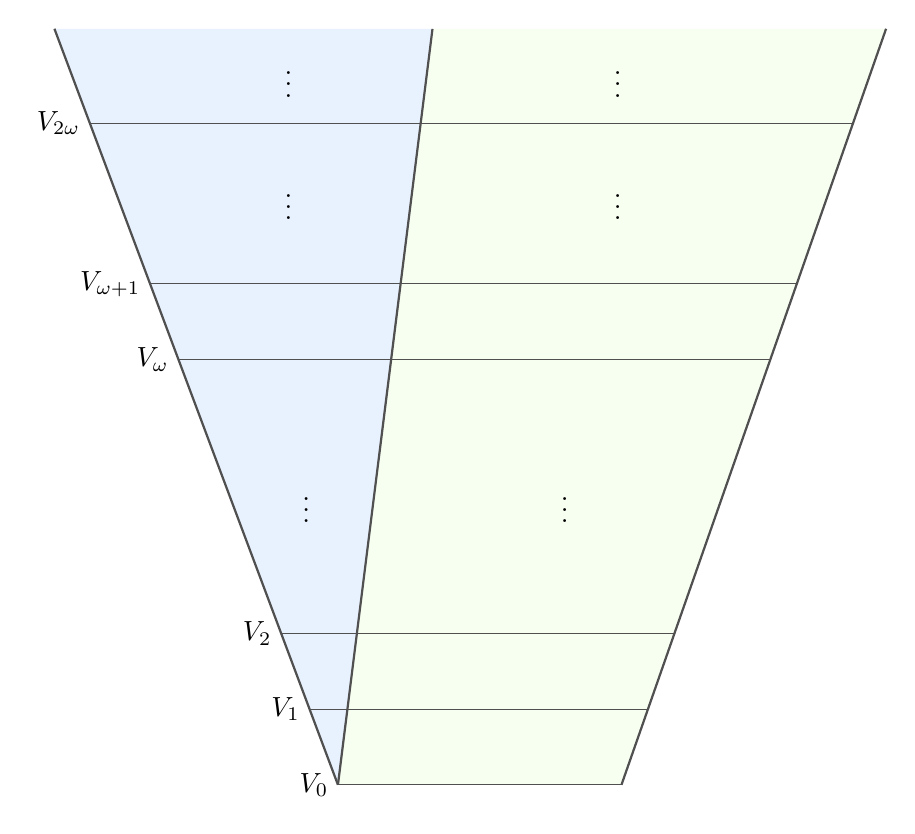
\begin{tikzpicture}[scale=1.2]
    % Define colors
    \definecolor{purecolor}{RGB}{210, 230, 255}
    \definecolor{impurecolor}{RGB}{230, 255, 210}
    \definecolor{linecolor}{RGB}{80, 80, 80}

    % Define the straight boundary points
    \coordinate (bottomL) at (-3, 0);
    \coordinate (topL) at (-6, 8);
    \coordinate (bottomR) at (0, 0);
    \coordinate (topR) at (2.8, 8);

    % Define y-coordinates for each level
    \def\yV{0}
    \def\yI{0.8}
    \def\yII{1.6}
    \def\ydots{3}
    \def\yomega{4.5}
    \def\yomegaplus{5.3}
    \def\ydotstwo{6.5}
    \def\ytwoomega{7}

    % Calculate x-coordinates on the straight boundaries for each level
    % Left boundary: interpolate between (-3,0) and (-6,8)
    \coordinate (V0L) at ({-3 + (-3) * \yV / 8}, \yV);
    \coordinate (V1L) at ({-3 + (-3) * \yI / 8}, \yI);
    \coordinate (V2L) at ({-3 + (-3) * \yII / 8}, \yII);
    \coordinate (VdL) at ({-3 + (-3) * \ydots / 8}, \ydots);
    \coordinate (VwL) at ({-3 + (-3) * \yomega / 8}, \yomega);
    \coordinate (Vw1L) at ({-3 + (-3) * \yomegaplus / 8}, \yomegaplus);
    \coordinate (Vd2L) at ({-3 + (-3) * \ydotstwo / 8}, \ydotstwo);
    \coordinate (V2wL) at ({-3 + (-3) * \ytwoomega / 8}, \ytwoomega);

    % Right boundary: interpolate between (0,0) and (2.8,8)
    \coordinate (V0R) at ({0 + 2.8 * \yV / 8}, \yV);
    \coordinate (V1R) at ({0 + 2.8 * \yI / 8}, \yI);
    \coordinate (V2R) at ({0 + 2.8 * \yII / 8}, \yII);
    \coordinate (VdR) at ({0 + 2.8 * \ydots / 8}, \ydots);
    \coordinate (VwR) at ({0 + 2.8 * \yomega / 8}, \yomega);
    \coordinate (Vw1R) at ({0 + 2.8 * \yomegaplus / 8}, \yomegaplus);
    \coordinate (Vd2R) at ({0 + 2.8 * \ydotstwo / 8}, \ydotstwo);
    \coordinate (V2wR) at ({0 + 2.8 * \ytwoomega / 8}, \ytwoomega);

    % Fill the impure hierarchy (total area minus pure triangle)
    \fill[impurecolor, opacity=0.3] (bottomL) -- (bottomR) -- (topR) -- (-2, 8) -- cycle;

    % Fill the pure hierarchy (triangular part with tip at bottom left)
    \fill[purecolor, opacity=0.5] (bottomL) -- (-2, 8) -- (topL) -- cycle;

    % Draw the straight boundary lines
    \draw[thick, linecolor] (bottomL) -- (topL);
    \draw[thick, linecolor] (bottomR) -- (topR);

    % Draw horizontal level lines (only for labeled stages)
    \draw[linecolor] (V0L) -- (V0R);
    \draw[linecolor] (V1L) -- (V1R);
    \draw[linecolor] (V2L) -- (V2R);
    \draw[linecolor] (VwL) -- (VwR);
    \draw[linecolor] (Vw1L) -- (Vw1R);
    \draw[linecolor] (V2wL) -- (V2wR);

    % Draw the pure hierarchy boundary (diagonal from bottom left tip)
    \draw[thick, linecolor] (bottomL) -- (-2, 8);

    % Add level labels on the left
    \node[left] at (V0L) {$V_0$};
    \node[left] at (V1L) {$V_1$};
    \node[left] at (V2L) {$V_2$};
    \node[left] at (VwL) {$V_\omega$};
    \node[left] at (Vw1L) {$V_{\omega+1}$};
    \node[left] at (V2wL) {$V_{2\omega}$};

    % Add dots for skipped stages (inside the hierarchy)
    \node at ({-3 + (-3) * 2.5 / 8 + 0.6}, 3) {$\vdots$};
    \node at ({-3 + (-3) * 3 / 8 + 0.6}, 6.2) {$\vdots$};
    \node at ({-3 + (-3) * 3 / 8 + 0.6}, 7.5) {$\vdots$};

    % Add dots on the right side too (inside the hierarchy)
    \node at ({0 + 2.8 * 0 / 8 - 0.6}, 3) {$\vdots$};
    \node at ({0 + 2.8 * 1.6 / 8 - 0.6}, 6.2) {$\vdots$};
    \node at ({0 + 2.8 * 1.6 / 8 - 0.6}, 7.5) {$\vdots$};

\end{tikzpicture}
% \end{document}

  }
\end{wrapfigure}

But we don't stop there.
After all the stages $V_0, V_1, V_2, \ldots$,
there is another stage $V_{\omega}$ (``$V$ omega'').
$V_\omega$ contains all sets that have appeared at any earlier stage.
That is,
$V_{\omega}$ is the union of all earlier stages:
\[
  V_{\omega} = \bigcup_{k < \omega} V_{k}.
\]
While all sets in the sequence $V_0,V_1, V_2, \ldots$ are finite,
$V_{\omega}$ has infinitely many elements.

From $V_{\omega}$,
we can form yet further sets by repeating the previous recipes.
At stage $V_{\omega + 1}$,
we collect all the subsets of $V_{\omega}$.
(Many of these are infinite and thus didn't appear at any earlier stage.)
That is,
$V_{\omega + 1} = \mathcal{P}(V_{\omega})$.
We then form $V_{\omega + 2} = \mathcal{P}(V_{\omega + 1})$,
and so on.
After all the stages $V_{\omega}, V_{\omega + 1}, V_{\omega + 2}, \ldots$,
there is another stage $V_{\omega + \omega}$, or $V_{\omega \cdot 2}$.
It contains all sets that have appeared at any earlier stage:
$V_{\omega \cdot 2} = \bigcup_{k < \omega} V_{\omega + k}$.
From $V_{\omega \cdot 2}$,
we construct $V_{\omega \cdot 2 + 1}$, $V_{\omega \cdot 2 + 2}$, \ldots by taking power sets.
Then we construct $V_{\omega \cdot 3}$ by taking the union of all earlier stages.
And so on and on.

And we don't stop there.
After all the stages $V_{\omega}, \ldots, V_{\omega \cdot 2}, \ldots, V_{\omega \cdot 3}, \ldots$,
there is another stage $V_{\omega\cdot \omega}$, or $V_{\omega^{2}}$,
where we take the union of all previous stages.
From this,
we construct further stages by taking power sets and unions.
Eventually,
we reach $V_{\omega^{3}}$,
then $V_{\omega^{4}}$, etc.
Then we take the union of all these stages to get $V_{\omega^{\omega}}$,
and so on and on,
through $V_{\omega^{\omega^\omega}}$,
through stages with infinitely high towers of $\omega$,
and much, much further.
The cumulative hierarchy is \textit{vast}.

\begin{exercise}
  Consider the pure hierarchy.
  How many sets are in $V_{3}$?
  How many are in $V_4$?
\end{exercise}

\begin{exercise}
  Is the cardinality of $V_{\omega\!+\!1}$ greater than the cardinality of $V_{\omega}$?
\end{exercise}

% ** Language of set theory

Let's now try to axiomatize this conception of sets.
That is,
we'll try to find a set of sentences in a suitable first-order language
that describes the structure of the cumulative hierarchy.
The description I just gave,
with its `and so on's and `after all these stages' can't be directly translated into first-order logic.
We have to take a more indirect approach.

The most popular axiomatization of set theory is \emph{ZFC},
for `Zermelo-Fraenkel set theory with the Axiom of Choice'.
Its only primitive concept is the membership relation.
So we have a single non-logical symbol:
the binary predicate symbol `$\in$'.
From this,
other concepts are defined.
For example,
we can define the subset relation $\subseteq$ as follows:

\begin{quote}
   $t_1 \subseteq t_2$ abbreviates $\forall x (x \in t_1 \rightarrow x \in t_2)$.
\end{quote}

% \begin{itemize}
% \item $x \subseteq y$ means $\forall z (z \in x \rightarrow z \in y)$
% \item $x \cup y$ means $\{ z : z \in x \lor z \in y \}$
% \item $x \cap y$ means $\{ z : z \in x \land z \in y \}$
% \item $\bigcup x$ means $\{ z : \exists y (y \in x \land z \in y) \}$, the union of all sets in $x$.
% \item $P(x)$ means the power set of $x$, i.e. $\{ y : y \subseteq x \}$.
% \end{itemize}

Let's go through the axioms of ZFC.
The quantifiers are assumed to range over the pure sets.
Our first axiom is known as the axiom of \emph{extensionality}.

\begin{axioms}
  Z1 & $\forall x\forall y( (\forall z(z\in x\leftrightarrow z\in y)) \to x=y ).$
\end{axioms}

This says that a set is determined by its elements:
no two sets have the same elements.
Unlike Frege's Axiom V,
Z1 doesn't imply that
for any formula $A(x)$ there is a corresponding set $\{ x : A(x) \}$.
Instead of this unrestricted comprehension principle,
we have a more restricted principle,
called the \emph{separation axiom}.
It's actually a schema:

\begin{axioms}
  Z2 & $\forall y \exists z \forall x( x\in z \leftrightarrow ( x\in y \land A(x)))$
\end{axioms}
\noindent%
This says that for any set $y$ and any formula $A(x)$,
there is a set $z$ that contains just those elements of $y$ of which $A(x)$ is true.
That is,
provided that we already have a set $y$,
we can use any formula to carve out a subset of $y$
containing those elements of $y$ of which the formula is true.

The next axiom postulates the existence of the empty set,
the base level of the hierarchy.

\begin{axioms}
   Z3 & $\exists x\forall y(y\notin x).$
\end{axioms}
\noindent%
This says that there is something (a set) that has no elements.
By the extensionality axiom,
there is only one such thing.
It's convenient to have a name for it: `$\emptyset$'.
But `$\emptyset$' isn't officially part of the language.
The only singular terms in the language of set theory are variables.
So we can't say that `$\emptyset$' is shorthand for some more complex term in the language,
in the way we could treat `3' as shorthand for `s(s(s(0)))'.
What we can do instead is give a \emph{contextual} or \emph{syncategorematic} definition of `$\emptyset$',
as follows:

\begin{axioms}
  & $A(\emptyset)$ abbreviates $\exists x(\forall y\, y\notin x\, \land A(x))$.
\end{axioms}
%
Here, $A(x)$ is an expression with one free variable $x$,
and $A(\emptyset)$ is that expression with `$\emptyset$' in place of $x$.
For example, consider the expression
\[
  \forall x(\emptyset \subseteq x).
\]
By the convention for $\emptyset$,
it is shorthand for
\[
  \exists z(\forall y(y\notin z) \land \forall x(z \subseteq x)).
\]
By the convention for $\subseteq$, this is in turn shorthand for
\[
  \exists z(\forall y(y\notin z) \land \forall x\forall v(v \in z \to v \in x)).
\]

The same trick is needed to talk about operations on sets.
To define the union $\cup$ operation,
for example,
we need to find a formula that is true of sets $x,y$, and $z$
iff $z$ is the union of sets $x$ and $y$.
Such a formula is not hard to find:
\[
  \forall v(v\in x \lor v \in y \leftrightarrow v \in z).
\]
With this, we can give a contextual definition of `$\cup$':

\begin{axioms}
  &
  $A(t_{1} \cup t_{2})$ abbreviates
  $\exists x(\forall y(y\in t_1 \lor y \in t_2 \leftrightarrow y \in x) \land A(x))$,
\end{axioms}
%
\noindent%
where $x$ and $y$ do not occur in $A$.

We can similarly define the intersection operation $\cap$:
\begin{axioms}
  &
  $A(t_{1} \cap t_{2})$ abbreviates
  $\exists x(\forall y(y\in t_1 \land y \in t_2 \leftrightarrow y \in x) \land A(x))$.
\end{axioms}

\begin{exercise}
  Give contextual definitions of $\bigcup t$ and $\mathcal{P}(t)$.
  $\bigcup t$ is the union of all sets in $t$;
  $\mathcal{P}(t)$ is the set of all subsets of $t$.
\end{exercise}

% \begin{axioms}
%   &
%   $A(\bigcup t)$ abbreviates
%   $\exists x(\forall y(\exists z(z\in t \land y\in z) \leftrightarrow y \in x) \land A(x))$.
% \end{axioms}

The next two axioms guarantee that
for every set $x$,
there is a set $\bigcup x$ comprising all elements of elements of $x$,
and a set $\mathcal{P}(x)$ comprising all subsets of $x$.
Z4 is the \emph{union axiom},
Z5 the \emph{powerset axiom}.

\begin{axioms}
  Z4 & $\forall x\exists u\forall y(y\in u \leftrightarrow \exists z(z\in x \land y\in z)).$\\
  Z5 & $\forall x\exists p\forall y(y\in p \leftrightarrow y\subseteq x).$
\end{axioms}

% Z4 says that
% whenever we have a set x of sets,
% we may form a set from all the elements of those sets, i.e. the union $\bigcup x$.
% Z5 says that
% whenever we have a set x, we may form the set of all its subsets, i.e. the power set P(x).

Next,
we have the \emph{pairing axiom}:
%
\begin{axioms}
   Z6 & $\forall x\forall y \exists z\forall v(v\in z \leftrightarrow (v=x \lor v=y))$
\end{axioms}
%
\noindent%
This says that
for any sets $x,y$
there is a set $\{x,y\}$ that contains exactly $x$ and $y$.
This is needed, for example,
to ensure that $x \cup y$ exists whenever $x$ and $y$ exist:
the pairing axiom gives us $\{x,y\}$,
from which we get $x \cup y = \bigcup \{x,y\}$ by Z4.

The sets $x$ and $y$ in Z6 needn't be different.
For the case where $x = y$,
the axiom says that
for every set $x$ there is a set $\{x,x\}$ = $\{ x \}$ that contains exactly $x$.
This is called the \emph{singleton} set of $x$.
We'll help ourselves to $\{t\}$ as a contextually defined term:

\begin{quote}
  $A(\{ t \})$ abbreviates
  $\exists x(\forall y(y\in x \leftrightarrow y = t) \land A(x))$.
\end{quote}

We make use of this abbreviation in our next axiom,
the \emph{axiom of infinity}:

\begin{axioms}
  Z7 & $\exists x( \emptyset\in x \land \forall y(y\in x\to y\cup\{y\}\in x)).$
\end{axioms}

\noindent%
Without the axiom of infinity,
we couldn't guarantee the existence of any infinite set.
In the next section,
we'll see that the set $x$ whose existence is guaranteed by Z7
can be understood as the set $\mathbb{N}$ of natural numbers.

\begin{exercise}
  List three members of the set whose existence is guaranteed by Z7.
\end{exercise}

Next,
we have the axiom of \emph{foundation} (or \emph{regularity}).
It ensures that every set (every object in the domain) is part of the cumulative hierarchy.
Consider any nonempty set $x$.
The elements of $x$ are other sets.
If $x$ is in the cumulative hierarchy,
then its elements must have appeared at earlier stages in the construction,
and there must be some stage at which the first of them appeared.
Let $y$ be one of these earliest elements.
Since all elements of $y$ appear strictly before $y$,
it follows that 
none of the elements of $y$ are elements of $x$.
That is,
every nonempty set $x$ of sets must have an element $y$ that is disjoint from $x$:

\begin{axioms}
  Z8 & $\forall x( x\neq\emptyset \to \exists y(y \in x \,\land\, x\cap y = \emptyset ))$
\end{axioms}

There are two more axioms.
Next is the \emph{axiom of replacement},
due to Abraham Fraenkel.
It is motivated by the observation that
the naive comprehension principle only seems to go wrong
in cases where the formula $A(x)$ from which it allows
defining a set $\{ x \,:\, A(x) \}$ is true of every set,
or of things of which there are as many as there are sets.
For example,
Russell's $x \not\in x$ is true of all the sets.
Objects of which there are as many as there are sets are sometimes said to form a \emph{proper class}.
(This concept is formalized in some extensions of ZFC,
such as the von Neumann-Bernays-Gödel set theory NBG.)
In essence,
the axiom of replacement says that
if there are no more objects of a certain kind than there are members of some set $x$,
then these objects also form a set.
After all,
they can't form a proper class if there are no more of them than there are members of $x$,
which is known to be a set.

To see how this may be used,
suppose that we have a construction
that defines a set $s_{n}$ for each natural number.
So there are as many sets $s_{0}, s_{1}, s_{2}, \ldots$ as there are natural numbers.
If we identify the natural numbers with the elements of the set whose existence is guaranteed by Z7,
we know that the natural numbers form a set.
The replacement axiom allows us to conclude that
the $s_0, s_1, s_2, \ldots$ also form a set.
It is called `replacement' because
it allows replacing all members $i$ of a known set by other things $f(i)$.

Let's review how we compare the sizes of infinite collections.
By the standards of section~\ref{sec:cardinalities},
a set $x$ is no larger than a set $y$
iff there is an injective function from $x$ to $y$:
a function that maps each element of $x$ to an element of $y$,
without mapping different elements of $x$ to the same element of $y$.
In set theory,
we don't have functions as separate objects.
But we can simulate them by sets.
Since functions are fully determined by which outputs they return for which inputs,
we can identify them with sets of input-output pairs.
For example,
the square function on the natural numbers would be identified with
the set of ordered pairs $\t{0,0}$, $\t{1,1}$, $\t{2,4}$, $\t{3,9}$, etc.

To complete this definition,
we need to provide a set-theoretic surrogate for the concept of an ordered pair.
An ordered pair $\t{x,y}$ isn't simply the set $\{ x,y \}$:
we want to distinguish $\t{2,4}$ from $\t{4,2}$.
In general,
ordered pairs $\t{x_1,y_1}$ and $\t{x_2,y_2}$ are identical iff
$x_1=x_2$ and $y_1=y_2$.
Can we find set-theoretic constructs that satisfy this condition?
Easy.
The standard construction, due to Kazimierz Kuratowski,
identifies $\t{x,y}$ with the set $\{ \{ x \}, \{ x,y \} \}$.
You can easily show that,
on this definition,
$\t{x_1,y_1} = \t{x_2,y_2}$ iff $x_1=x_2$ and $y_1=y_2$.

\begin{exercise}
  Find another set-theoretic construction of $\t{x,y}$ that satisfies the identity condition for ordered pairs.
\end{exercise}

Return to the axiom of replacement.
We want to use the axiom show that
certain objects form a set,
given that there are no more of them than there are members of some other set.
Unfortunately,
we can't assume in this context
we have already established the existence of any functions
from the objects to the other set.
(If we knew that
there is a set of ordered pairs $\t{x,y}$ in which each
of our objects figures as a first member,
we could infer that the objects form a set by the axioms of union and separation:
we wouldn't need replacement).

Instead of invoking functions,
the replacement axiom therefore uses \emph{formulas} to express that
there is a functional relationship.
First, a convenient abbreviation:
\begin{quote}
   $\exists! x A(x)$ abbreviates $\exists x (A(x) \land \forall y ({A(y) \to y\!=\!x}))$,
\end{quote}
$\exists!x A(x)$ says that there is exactly one $x$ such that $A(x)$.
So $\forall x\exists! y A(x,y)$ says that
$A(x,y)$ expresses a functional relationship:
it relates each $x$ to exactly one $y$.
If there is such a functional relationship between
the members of some set $v$ and some $y$s,
there can be no more $y$s than there are members of $v$.
The axiom of replacement, which is really an axiom schema, allows us to conclude that
there is a set $w$ that contains all these $y$s:

\begin{axioms}
    Z9 & $\forall v((\forall x(x \in v \to \exists!y A(x,y)) \to \exists w\forall x(x \in v \leftrightarrow \exists y(y \in w \land A(x,y)))))$
\end{axioms}

For applications of set theory,
Replacement is rarely needed.
But we need it to ensure that the cumulative hierarchy extends to $V_{\omega\!+\!\omega}$.
From Z1--Z8 (sometimes called \emph{Zermelo set theory} or Z),
we get $V_0, V_1, V_2, \ldots, V_{\omega}, V_{\omega\!+\!1}, V_{\omega\!+\!2}, \ldots$,
but we don't get to $V_{\omega\!+\!\omega}$.
With Replacement,
we can show that the set $\{ V_{\omega\!+\!n} : n \in \mathbb{N} \}$ exists.
$V_{\omega\!+\!\omega}$ is the union of this set.
To show that it exists,
we use Replacement with formula $A(x,y)$ saying that
$y$ is obtained from $V_{\omega}$
by $x$ applications of the power set operation.


Finally,
we have Zermelo's Axiom of Choice.
This says that if we have a set $x$ of non-empty sets,
then there is a set $y$ that contains exactly one element from each set in $x$.

\begin{axioms}
    Z10 & $\forall x[\forall z(z \in x \to z\neq\emptyset) \to \exists y \forall z(z \in x \to \exists! v(v \in z \land v \in y))]$ \\
\end{axioms}

Unlike the other axioms,
the Axiom of Choice states that a certain set exists
without describing how it can be constructed:
we are not told \emph{which} element of each set in $x$ is in $y$.
For this reason (as well as certain strange consequences in the theory of measures),
the axiom has long been controversial.
Nowadays,
it is generally accepted,
as many important mathematical results depend on it.

\begin{exercise}
  Prove from the axioms of ZFC that for any three things a,b,c, there is a set \{a,b,c\}.
\end{exercise}

\begin{exercise}
  Explain why the separation axiom implies that there is no set of all sets.
\end{exercise}

% An example of something that can be formalized in ZFC is the completeness theorem of the previous chapter.
% This requires interpreting the language, proofs, models, etc. in set theory.
% Models are set theoretic structures.
% So validity and entailment are really set-theoretic concepts.
% You may now appreciate how odd it is that they align so neatly with a finitary concept of derivability.

\section{Sets and numbers}\label{sec:ordinals}

The Axiom of Infinity draws attention to an infinite sequence of sets,
called the \emph{finite von Neumann ordinals},
or simply the \emph{finite ordinals}:

\begin{itemize*}
  \item $\emptyset$
  \item $\{ \emptyset \}$
  \item $\{ \emptyset, \{ \emptyset \} \}$
  \item $\{ \emptyset, \{ \emptyset \}, \{ \emptyset, \{ \emptyset \} \} \}$
  \item $\ldots$
\end{itemize*}
%
\noindent%
This sequence has the structure of the natural numbers.
We can think of $\emptyset$ as 0,
$\{ \emptyset \}$ as 1,
$\{ \emptyset, \{ \emptyset \} \}$ as 2,
and so on.
The successor of any number $n$ is $n \cup \{ n \}$.
(Note that,
conveniently,
each number $n$ in this construction has exactly $n$ elements.)

More formally,
we can use the finite ordinals to
define a model of arithmetical theories like $\mathrm{Th}(\Mod{N})$ and PA.
Recall that a model of a theory is
a structure consisting of a domain and an interpretation of the non-logical symbols
in which all sentences in the theory are true.
For a model of $\mathrm{Th}(\Mod{N})$,
we can choose as the domain the set $\omega$ of finite ordinals.
The interpretation function
maps the `0' symbol to $\emptyset$
and the successor symbol `$s$' to
the function that maps each set $x \in \omega$ to $x \cup \{ x \}$.
The standard recursive definitions of addition and multiplication
then determine the interpretation of `+' and `$\times$'.
(If $n$ and $m$ are in $\omega$,
$n + m$ will be the unique set in $\omega$ that
has exactly $n+m$ elements,
and $n \times m$ the unique set with $n \times m$ elements.)
This shows that the natural number structure can be embedded in the structure of sets.
The same is true for almost every mathematical structure.

There is more.
Suppose we read
\begin{itemize*}
  \item `$0$' as an abbreviation of `$\emptyset$',
  \item `$s(t)$' as an abbreviation of `$t \cup \{ t \}$',
  \item `$t_{1} + t_{2}$' and `$t_{1} \times t_{2}$' as abbreviations of the corresponding operations on sets,
\end{itemize*}
and we restrict all quantifiers in PA to range over $\omega$,
so that `$\forall x A$' becomes `$\forall x (x \in \omega \to A)$'
All axioms of PA are then provable in ZFC.
We say that PA is \textit{interpretable} in ZFC.
In general,
a theory $T$ is interpretable in ZFC if
there is a translation scheme of the kind I've sketched
under which all sentences in $T$ are provable in ZFC.

A wide range of mathematical theories are interpretable in ZFC.
In that sense,
ZFC is \emph{at least as strong} as these other theories:
whatever they can prove,
ZFC can prove as well
(if only under the appropriate translation scheme).

% (Indeed, it turns out that ZFC can prove purely arithmetical statements that PA
% cannot prove; e.g. Con(PA).)

I'm not going to prove that PA is interpretable in ZFC.
The proof isn't hard,
but a little fiddly.
To get a sense of what needs to be shown,
consider the second axiom of PA:

\begin{axioms}
  Q2 & $\forall x \, 0\! \not= \!s(x)$
\end{axioms}

Under the above translation scheme,
this turns into $\forall x (x \in \omega  \to (\emptyset \ne x \cup \{ x \}))$.
And that's easily provable in ZFC.

\begin{exercise}
  Sketch a proof of the translated Q2 axiom (from the axioms of ZFC).
\end{exercise}

% One of the earliest and most important applications of set theory is
% that it allows counting beyond infinity.
% I'll briefly describe how this works.

Let's now have a closer look at the finite ordinals.
They have some interesting properties.

For one,
every member of a finite ordinal is also a subset of it.
Sets of this kind are called \textit{transitive}.
That's because a transitive set $z$ is a set such that
whenever $x \in y$ and $y \in z$ then $x \in z$.

Another special property of the finite ordinals is that
% they are \emph{$\in$-well-ordered}.
they are \emph{linearly ordered by $\in$}:
any two members of $x$ are related one way or the other by $\in$.
I'll say, for short,
that the finite ordinals are \emph{$\in$-ordered}.

In ZFC,
the finite ordinals can be defined as
the transitive and $\in$-ordered sets with finitely many elements.
Now suppose we drop the finiteness condition.
Let's define an \emph{ordinal} as a transitive and $\in$-ordered set.
The finite ordinals are ordinals,
but they are not the only ones.
For example,
$\omega$, the set of finite ordinals, is itself an ordinal.
(As you can confirm,
it is transitive and $\in$-ordered.)
$\omega$ is an \emph{infinite ordinal}.
So is $\omega \cup \{ \omega \}$:
the set we get from $\omega$ by adding $\omega$ itself as an element.
Following our earlier definition of the successor relation,
we can see $\omega \cup \{ \omega \}$ as the ``successor'' of $\omega$.
The successor of $\omega \cup \{ \omega \}$ is $\omega \cup \{ \omega \} \cup \{ \omega \cup \{ \omega \} \}$,
and so on.

The ordinals form a \emph{transfinite} sequence.
If we identify the finite ordinals with the natural numbers,
the transfinite sequence of ordinals look like this:
\[
  0, 1, 2, \ldots, \omega, \omega\!+\!1, \omega\!+\!2, \ldots \omega\!+\!\omega, \ldots
\]

Like 0, $\omega$ is not the successor of any ordinal.
Infinite ordinals that are not successors are called \textit{limit ordinals}.
The next limit ordinal after $\omega$ is $\omega\!+\!\omega$,
or $\omega \cdot 2$.
It is the union of all ordinals $\omega\!+\!n$,
where $n$ is a finite ordinal.
The next limit ordinal after $\omega \cdot 2$ is $\omega \cdot 3$.
After all the limit ordinals $\omega \cdot n$
and all their successors
comes their union $\omega \cdot \omega$,
or $\omega^{2}$
-- another limit ordinal.
Much later we reach $\omega^{\omega}$, $\omega^{\omega^{\omega}}$, and so on.

The ordinals extend the idea of ``counting'' beyond the finite.
This has many mathematical applications.
Above,
I've used the ordinals to label stages in the cumulative hierarchy.
I used limit ordinals to label stages at which we take the union of the earlier stages,
and successor ordinals to label stages at which we take power sets.

% \begin{exercise}
%   Is the set $\{ 1, 2 \}$ transitive,
%   if 1 and 2 are construed as von Neumann ordinals?
% \end{exercise}

\begin{exercise}
  Show that $\omega$ is transitive and $\in$-ordered.
\end{exercise}

\begin{exercise}
  Show from the axioms of ZFC that every ordinal has a successor.
\end{exercise}

\begin{exercise}
  Is the set of all ordinals an ordinal?
\end{exercise}

The ordinals can also be used to
interpret the theory of cardinals that I outlined in the previous chapter.
Remember that two sets have the same cardinality
iff there is a bijection between them.
For finite sets,
cardinalities are naturally identified with natural numbers:
$\{ \text{Athens, Berlin, Cairo} \}$ has cardinality 3.
But what kind of thing is the cardinality of an infinite set?
In section~\ref{sec:cardinalities},
we gave them names:
we called them $\aleph_0$, $\aleph_1$, etc.
But I didn't say more about what these things might be.

The standard answer in contemporary set theory
identifies the cardinals with certain ordinals:
the cardinality of any set $x$ is defined as
\emph{the least ordinal that is equinumerous with $x$}.

For finite sets,
this yields the expected results.
$\{ \text{Athens, Berlin, Cairo} \}$ is equinumerous with $\{ \emptyset, \{ \emptyset \}, \{ \emptyset, \{ \emptyset \} \} \}$,
which is the ordinal 3.
So the cardinality of $\{$ Athens, Berlin, Cairo $\}$ is 3.
The cardinality of $\omega$ is $\omega$.
That's because $\omega$ is the least ordinal that is equinumerous with $\omega$.
Since $\omega$ is countably infinite,
and we defined $\aleph_{0}$ as the cardinality of any countably infinite set,
this means that $\omega = \aleph_0$.

Beyond $\aleph_{0}$,
things get interesting.
The cardinality of $\omega\!+\!1$ is still $\aleph_{0}$.
Remember that $\omega\!+\!1$ is $\omega \cup \{ \omega \}$:
it is $\omega$ with one extra element.
If you add a single element to a countably infinite set,
you always get another countably infinite set.
So $\omega\!+\!1$ is equinumerous with $\omega$.
Since the cardinality of a set is the \emph{least} ordinal equinumerous with it,
the cardinality of $\omega\!+\!1$ is $\omega$ (a.k.a. $\aleph_0$).

After $\omega$,
the \emph{ordinal numbers} and the \emph{cardinal numbers} diverge.
$\omega$ is both an ordinal and a cardinal.
But $\omega\!+\!1$ is only an ordinal.
We've introduced `$\aleph_1$' to name the next cardinal after $\aleph_0$.
By our current definition,
$\aleph_1$ is first ordinal in the transfinite sequence of ordinals
that is not equinumerous with $\omega$.
It comes surprisingly late.
It's not $\omega\!+\!1$,
or $\omega \cdot 2$, or $\omega^{2}$, or $\omega^{\omega}$,
or $\omega^{\omega^{\omega}}$.
All of these are equinumerous with $\omega$.
$\aleph_{1}$ comes much later.
And yet we know,
from Cantor's theorem,
that there are infinitely many different cardinalities.
Indeed,
for every ordinal $\kappa$,
there is a distinct cardinal $\aleph_{\kappa}$,
which is itself an ordinal!

By Cantor's theorem,
the cardinality of $\mathcal{P}(\omega)$ is greater than $\aleph_0$.
How much greater?
Cantor conjectured, but was unable to prove, that
the cardinality of $\mathcal{P}(\omega)$ is $\aleph_1$.
Since $\mathcal{P}(\omega)$ is equinumerous with the set of real numbers $\mathbb{R}$,
which is also known as the \emph{continuum},
Cantor's conjecture was that
there is no set whose cardinality is strictly between that of the natural numbers
and that of the real numbers.
This became known as the \emph{continuum hypothesis}.

In 1938,
Gödel proved that the continuum hypothesis is consistent with ZFC
(assuming ZFC itself is consistent):
it can't be disproved from the axioms of ZFC.
In 1963,
Paul Cohen showed that the negation of the continuum hypothesis is also consistent with ZFC
(assuming ZFC is consistent).
So the continuum hypothesis can be neither proved nor disproved in ZFC.

I find this odd.
Take the set of real numbers $\mathbb{R}$.
We know that this set is uncountable.
We can get a countable set by
removing sufficiently many elements from $\mathbb{R}$.
Can we also remove elements from $\mathbb{R}$
so that we get a set that's still uncountable, but smaller than $\mathbb{R}$?
I would expect this simple question to have a definite answer.
But it can't be answered from the standard axioms of set theory.
We could, of course, add the continuum hypothesis as a further axiom.
But we could equally add its negation.
Neither leads to a contradiction.

Early set theorists assumed that
all questions about pure sets have definite answers that
can be established by an extended kind of logic.
The status of the continuum hypothesis casts doubt on this picture.
By now,
hundreds of other statements are known that
can neither be proved nor disproved in ZFC.
We can investigate structures in which they hold
and structures in which they fail.
Perhaps there is no ``true'' structure of sets after all.
When we describe the cumulative hierarchy,
we seem to describe a unique structure.
We say that $V_{\omega+2}$ contains \textit{all subsets} of $V_{\omega+1}$.
But we can't tell whether
these subsets include sets with a cardinality between $\aleph_0$ and the continuum.
If the concept of `all subsets' has a definite meaning,
this meaning seems impossible to pin down.

\section{Unintended models, again}

In section~\ref{sec:arithmetic},
we looked at non-standard models of Q:
models in which all axioms of Q are true
but whose structure is clearly not that of the natural numbers.
I didn't emphasize it at the time,
but Peano Arithmetic also has non-standard models.
These are harder to construct directly.
But we know that they exist,
from the compactness theorem.

\begin{theorem}{}{nonstandardPA}
  There are non-standard models of Peano Arithmetic.
\end{theorem}
\begin{proof}
  \emph{Proof.}
  Let $c$ be an individual constant other than 0.
  Let $\Gamma$ be the set of sentences consisting of
  the axioms of PA together with
  all the sentences
  \[
    c \ne 0, c \ne s(0), c \ne s(s(0)), \ldots.
  \]
  Every finite subset of $\Gamma$ is true in the standard model of arithmetic:
  just interpret $c$ as a sufficiently large natural number.
  By the compactness theorem,
  $\Gamma$ has a model.
  All axioms of PA are true in this model.
  But the object denoted by $c$ (in this model) can't be a natural number:
  it lies outside the number sequence 0,1,2,3, etc.
  \qed
\end{proof}

Intuitively,
Peano Arithmetic doesn't ``know'' that
there are no numbers besides 0,1,2,3, etc.:
its axioms are compatible with the existence of further numbers.
We know from theorem~\ref{thm:non-standard-arithmetic} that
there's no way to add the missing information to PA,
in the form of further axioms:
even the set of all truths in the language of arithmetic, $\mathrm{Th}(\Mod{N})$,
has non-standard models.

\begin{exercise}
  PA rules out structures in which
  the ``non-standard numbers'' form either a loop or a second chain $a, s(a), s(s(a)), \ldots$.
  What else could a non-standard model look like?
\end{exercise}

Are there also non-standard models of ZFC?
Let's first clarify the standard model.
A model of ZFC consists of a set $D$ of objects
and an interpretation function $I$
that assigns some relation on $D$ to the symbol `$\in$'.
In the \emph{intended} model,
$D$ is the set of all sets,
and $I$ maps `$\in$' to \ldots\,
Wait.
There is no set of all sets!

In a sense,
every model of ZFC is a non-standard model.
For every model has a set as its domain,
but there is no set of all sets.
The real sets form a proper class.

The problem is that
we've formalized our semantic concepts in set-theoretic terms.
We've define models as set-theoretic structures.
The intended interpretation of ZFC can't be formalized in this way.

You may wonder how ZFC can have models in our set-theoretic sense at all.
In any set-theoretic model of ZFC,
the domain is a set,
but ZFC entails that there is no set of all sets.
We can strengthen this puzzle.
Let's take for granted that ZFC is consistent.
By the completeness theorem,
it follows that ZFC has a model.
By the (downward) Löwenheim-Skolem theorem,
it follows from this
that ZFC has a \emph{countable} model.
Call it $\Mod{M}$.
The domain of $\Mod{M}$ contains only countably many objects.
Yet all sentences in ZFC are true in $\Mod{M}$,
including sentences saying that
there are uncountably many things in $\mathcal{P}(\omega)$,
even more in $\mathcal{P}(\mathcal{P}(\omega))$, and so on.
This is known as ``Skolem's Paradox''.

It's not a real paradox.
A set $x$ is countable if
there is an injective function from  $x$ to $\omega$;
$x$ is uncountable if there is no such function.
ZFC proves that some $\mathcal{P}(\omega)$ is uncountable by proving that
there is no injective function from $\mathcal{P}(\omega)$ to $\omega$.
Remember that functions are represented as sets of ordered pairs.
To say that there is an injective function from $x$ to $\omega$ is to say that
there is a set $f$ of pairs $\t{y,n}$ such that
for each $y \in x$ there is exactly one $n \in \omega$ for which $\t{y,n} \in f$,
and for each $n \in \omega$ there is at most one $y \in x$ for which $\t{y,n} \in f$.
ZFC proves that there is no such set $f$ for $x = \mathcal{P}(\omega)$.
In the countable model $\Mod{M}$,
there may, in fact, be a bijection between the objects denoted by $\omega$ and $\mathcal{P}(\omega)$.
That is,
we may be able to construct such a bijection.
But it need not be an object in the domain of $\Mod{M}$.
If it is not,
the statement that there is no bijection of the given type is \emph{true} in $\Mod{M}$.

There is still a puzzle, however.
It is related to the puzzle from the end of the previous section.
How do we manage to latch onto the set-theoretic universe?
We could program an AI to interpret the language of ZFC in a countable model.
The AI would \emph{say} that there are uncountably many sets.
It would say all the right things.
But its conception of sets would seem to be radically different from ours.
For we can see that
there are, in fact, only countably many of the things it calls `sets'.
Given that this is possible,
how can we be sure that we are not equally mistaken about the true sets?
How do we know that
there isn't an outside perspective from which
one can see that
there only countably many of the things we call `sets'?

\begin{exercise}
  Explain why every model of ZFC has an infinite domain.
\end{exercise}

% Things don't look much clearer if we go second-order, as long as the
% second-order quantifiers are interpreted as ranging over sets. A model still
% consists of a set of things over which the quantifiers range. The second-order
% quantifiers range over sets of these things. These sets are sets according to
% the ambient theory that describes the models. They aren't among the things the
% interpreted theory would call "sets". Which second-order statements are true now
% depends on the modelling set theory.

% This also suggests that the higher-order characterisations or numbers etc. that
% seem categorical may not really be pinning down the relevant structures, if we
% adopt a set-theoretic interpretation of higher-order logic. We'd need to ensure
% that the ambient set theory has a definite interpretation.

% A way to resolve this would be to give a non-set theoretic interpretation of
% higher-order logic.


%%% Local Variables:
%%% mode: latex
%%% TeX-master: "logic3.tex"
%%% End:
